\chapter{Number Systems}
\chaplabel{numbers}

This chapter introduces the concepts of different numbering systems that
are relevant to microcontrollers.

\section{Decimal Numbers}
The standard number system used by humans is based on 10. This logically flows 
the usual numbers of fingers or toes humans have. When counting in the base 10 (decimal) we 
start at 0, count up to 9, then run out of numbers 
to use. When runs out of numbers, we put a number to the left of the column we were counting
in, and then start over at zero again which gives us the number 10. A more clear way to count 
would be to count from 00 to 09, then increment the left digit and start the right digit back
at 0. This can be continued until 99 is reached. But now we have a model to follow. If a 
column gets to 9, we increment a column to the left and start the current column over at 0. 
This leads to the number 100. This concept can be continued forever.

When given a particular number, 3254, in decimal the value is calculated as
\begin{equation}
	3254 = 3\cdot1000 + 2\cdot100 + 5\cdot10 + 4
\end{equation}
It could also be represented as
\begin{equation}
	3254 = 3\cdot10^3 + 2\cdot10^2 + 5\cdot10^1 + 4\cdot10^0
\end{equation}
This is the basis for a positional number system.

\section{Binary Numbers}
Computers run a base 2 system, also known as binary. This means that we only have two options 
at each position, 1 or 0, instead of the 10 available in the decimal system. However, counting
is done in the same way, when you run out of symbols, increment the position to the left and 
then start over at zero in the current position.

Binary numbers are also positional so a number like 1011 is 
\begin{equation}
	1011 = 1\cdot2^3 + 0\cdot2^2 + 1\cdot2^1 + 1\cdot2^0 = 11_{10}
\end{equation}
where $11_{10}$ indicates that the number 11 is base 10.

The maximum value a binary number can have is determined by the number of bits it has. The formula is: 
\begin{equation}
	V_{max} = 2^n - 1
\end{equation}
where n is the number of bits. For example, an 8 bit number has a maximum value of $2^8 - 1 = 255$.

\section{Hexadecimal Numbers}
\begin{sloppypar}
The problem for humans is that we have a very difficult time reading binary numbers. Especially once the
numbers get long such as $11101101010010110101_2$. The first thing we can do to improve intelligibility is to 
put a space in every 4 digits so that we aren't completely bowled over by all the digits. This gives us
$1110~1101~0100~1011~0101_2$. This is better but still leaves some challenges. Someone pointed out that since
4~bits can have 16 different values, what if each 4~bits (also called a nibble) was represented by a single
base 16 number. Base 16 is called hexadecimal. It has the problem that it runs out of digits once we get to 
10, so it was decided to simply start on the alphabet so $10_{10}$ is $A_{16}$, $11_{10}$ is $B_{16}$, and so forth. Now 
the cumbersome binary number we've been playing with can be represented as $ED4B5_{16}$. 
\end{sloppypar}

A comparison of the different numbering system representations of 0 through $15_{10}$ are shown in 
Table~\ref{table:numsystems}.

\begin{table}[!ht]
	\centering
	\begin{tabular}{c c c}
		\hline
		Decimal & Binary & Hexadecimal \\ 
		\hline
		00 & 0000 & 0 \\
		01 & 0001 & 1 \\
		02 & 0010 & 2 \\
		03 & 0011 & 3 \\
		04 & 0100 & 4 \\
		05 & 0101 & 5 \\
		06 & 0110 & 6 \\
		07 & 0111 & 7 \\
		08 & 1000 & 8 \\
		09 & 1001 & 9 \\
		10 & 1010 & A \\
		11 & 1011 & B \\
		12 & 1100 & C \\
		13 & 1101 & D \\
		14 & 1110 & E \\
		15 & 1111 & F \\
		\hline
	\end{tabular}
	\caption{Decimal, binary, and hexadecimal numbers align as shown in this table.}
	\label{table:numsystems}
\end{table}

\section{Binary Background}
The reasons for this stem from early computers 
using switches (relays) as their basic computing elements and the fact that telling the 
difference between a ``high" voltage and a ``low" voltage is easier to do than to differentiate
10 different voltages. It also allows for a gap between high and low that creates some 
immunity to noise called the \href{https://3.bp.blogspot.com/-7GOaQqAncoU/VelAErlx5gI/AAAAAAAARLE/kITWaG8LAws/s1600/noise%2Bmargin.png}{noise margin}. 
The figure linked to labels noise margin at NM which indicates how much (in volts) the signal coming
from the source on the left can be degraded and still be recognized as a high or low. The other 
cool thing about digital signals is that each device the signal passes through removes
all noise.

\section{Converting Between Bases}
\subsection{Binary to Decimal}
Converting to decimal is straightforward since we can simply sum each digit multiplied by the 
power of 2 it represents. 
\begin{equation}
	\label{eq:bin2dec}
	V_{10} = \sum_{i=0}^p d_i \cdot 2^i
\end{equation}
In Equation~\ref{eq:bin2dec} the $p$ digits, $d_i$, of the binary number are summed from right 
to left while being multiplied by the power of 2 they represent. As an example, convert 
1011~0111 to decimal.
\begin{equation}
	\begin{split}
	V_{10} &= 1\cdot2^0 + 1\cdot2^1 + 1\cdot2^2 + 0\cdot2^3 + 1\cdot2^4 + 1\cdot2^5 + 0\cdot2^6 + 1\cdot2^7\\
		&= 1 + 2 + 4 + 0 + 16 + 32 + 0 + 128\\
		&= 183
	\end{split}
\end{equation}
I usually find it easiest to just remember the powers of two for each place and add them up.
\begin{equation}
	\overset{128}{1}\quad\overset{64}{0}\quad\overset{32}{1}\quad\overset{16}{1}\quad\overset{8}{0}\quad
	\overset{4}{1}\quad\overset{2}{1}\quad\overset{1}{1} = 1 + 2 + 4 + 16 + 32 + 128
\end{equation}

\subsection{Decimal to Binary}
Converting decimal numbers to binary involves dividing by 2 until the remainder is 0 or 1. The process
goes as follows:
\begin{enumerate}
	\item  Divide the number by 2. If the remainder is 1 then the least significant bit is 1 otherwise if the remainder is 0 
	(it was an even number) then the least significant bit is 0.
	\item \label{st:d2b2}Take the quotient from the previous step and divide by 2. The remainder is the next more significant bit in the binary representation.
	\item Repeat Step \ref{st:d2b2} until the quotient is 0.
\end{enumerate}

As an example, let's convert $11_{10}$ to binary. 
\begin{equation}
	\begin{aligned}
		11 \divisionsymbol 2 & = 5R1 &\rightarrow 1 &\mathrm{~(LSB)} \\
		5 \divisionsymbol 2 & = 2R1 &\rightarrow 1 \\
		2 \divisionsymbol 2 & = 1R0 &\rightarrow 0 \\
		1 \divisionsymbol 2 & = 0R1 &\rightarrow 1 & \mathrm{~(MSB)}
	\end{aligned}
\end{equation}
That means that $11_{10}$ is $1011_2$. As another example let us convert $20_{10}$ to binary.
\begin{equation}
	\begin{aligned}
		20 \divisionsymbol 2 & = 10R0 &\rightarrow 0 &\mathrm{~(LSB)}\\
		10 \divisionsymbol 2 & = 5R0  &\rightarrow 0 \\
		5 \divisionsymbol 2 &  = 2R1  &\rightarrow 1 \\
		2 \divisionsymbol 2 &  = 1R0  &\rightarrow 0 \\
		1 \divisionsymbol 2 &  = 0R1  &\rightarrow 1 & \mathrm{~(MSB)}
	\end{aligned}
\end{equation}
This shows that $20_{10}$ is $10100_2$.

\subsection{Binary and Hexadecimal}
For conversions between binary and hexadecimal I tend to use the table lookup method. After using it 
enough times you begin to memorize the conversions. In my head I'm usually converting from binary to 
decimal on each nibble and then converting decimal into hexadecimal. So if I see 0101 I remember it 
is 5 in decimal which is the same in hex. If I see 1010 I remember that it is $8 + 2 = 10$ which is 
one more than 9 so it is A in hex.

\section{Colors}
Colors for display on computers are represented as binary numbers. Colors are 24~bit which is broken
down into 3 8~bit numbers representing red, green, and blue (RGB). Eight bits give values over the 
range of 0 to 255 so colors are represented by 3 numbers such as (255, 0, 255) which gives a 
\textcolor[RGB]{255, 0, 255}{color like this}. It is good to note that (255, 255, 255) is white,
(0, 0, 0) is black, and (X, X, X) where all three numbers are the same is gray.

Sometimes colors are represented as a 6~digit binary number in hexadecimal form prefixed by 0x such 
as 0xFF00FF for the color we looked at previously. 

\section{ASCII}
Since computers operate using binary numbers, how do we get them to represent human languages? The method 
caught it is called \href{https://en.wikipedia.org/wiki/ASCII}{American Standard Code for Information Interchange (ASCII)}. Basically, 7~bit numbers
were mapped to letters, numbers, punctuation, symbols, and control characters. Some examples are A is 65, Z 
is 90, a is 97, z is 122, 0 is 48, 9 is 57. The most used control characters are carriage return (13 or \textbackslash r) and 
line feed (10 or \textbackslash n). Unix based operating systems (Linux, OS X) use line feed to indicate a new line. Windows
uses both (\textbackslash r\textbackslash n).

Look up an ASCII table online when you need to know the values.

\section{Adding and Subtracting Binary Numbers}
\subsection{Default method}

\subsubsection{Addition}
% addition method based on https://tex.stackexchange.com/a/96764
Calculate the binary sum $0001\;0011\;1101+0000\;1011\;0111$.
\begin{equation}
\begin{tikzpicture}[
    row 1/.style={font=\textsl,font=\scriptsize,black!85, %anchor=west,
        inner sep=1.5pt, row sep=-3pt},
    every node/.style={column sep=.5pt,row sep=1pt}]
    \matrix (m) [matrix of math nodes,
        nodes in empty cells,
        %nodes=draw
    ] 
    {
        &   &   &   &   &   & 1 & 1 & 1 & 1 & 1 & 1 &   &                   \\
        & 0 & 0 & 0 & 1 & 0 & 0 & 1 & 1 & 1 & 1 & 0 & 1 &[10mm] \\
    +   & 0 & 0 & 0 & 0 & 1 & 0 & 1 & 1 & 0 & 1 & 1 & 1 &  \\ 
        & 0 & 0 & 0 & 1 & 1 & 1 & 1 & 1 & 0 & 1 & 0 & 0 &  \\                                                  
    };

    \draw[-,color=black,semithick] (m-3-1.south west) -- (m-3-13.south east);

\end{tikzpicture}
\label{binary_integer_addition}
\end{equation}

\subsubsection{Subtraction}
Calculate the binary difference $0001\;0011\;1101-0000\;1011\;0111$.
\begin{equation}
\begin{tikzpicture}[
    every node/.style={column sep=.5pt,row sep=1pt}]
    \matrix (m) [matrix of math nodes,
        nodes in empty cells,
        %nodes=draw
    ] 
    {
        & 0 & 0 & 0 & \cancelto{0}{1} & \cancelto{10}{0} & 0 & 1 & 1 & \cancelto{0}{1} & \cancelto{\cancelto{10}{0}}{1} & \cancelto{10}{0} & 1 &[10mm] \\
    -   & 0 & 0 & 0 & 0 & 1 & 0 & 1 & 1 & 0 & 1 & 1 & 1 &  \\ 
        & 0 & 0 & 0 & 0 & 1 & 0 & 0 & 0 & 0 & 1 & 1 & 0 &  \\                                                  
    };

    \draw[-,color=black,semithick] (m-2-1.south west) -- (m-2-13.south east);

\end{tikzpicture}
\label{binary_integer_subraction}
\end{equation}


\subsection{Twos Complement method}

\begin{table}[!ht]
	\centering
	\begin{tabular}{S c}
		\hline
		{Decimal} & {Two's Complement} \\ 
		\hline
		7 & 0111 \\
		6 & 0110 \\
		5 & 0101 \\
		4 & 0100 \\
		3 & 0011 \\
		2 & 0010 \\
		1 & 0001 \\
		0 & 0000 \\
		-1 & 1111 \\
		-2 & 1110 \\
		-3 & 1101 \\
		-4 & 1100 \\
		-5 & 1011 \\
		-6 & 1010 \\
		-7 & 1001 \\
		-8 & 1000 \\
		\hline
	\end{tabular}
	\caption{This table shows the decimal and two's complement numbers for 4-bits.}
	\label{table:twoscomplement}
\end{table}


\section{Gray Codes}
When counting in binary, often times more than one bit changes as the number increments. This works fine
in the ideal world, but in the real world, the logic controlling each bit might be slightly different. This 
will cause one bit to change at a slightly different time than another bit. That causes glitches in the counting
that can be disruptive to the overall system. 

Take as an example a robot that represents the cardinal directions as binary integers as illustrated in Figure \ref{fig:nongraydir}.
\begin{figure}[!htb]
	\centering
	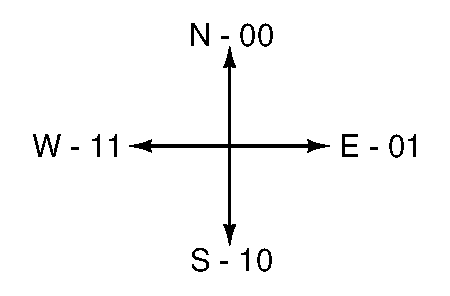
\includegraphics[scale=0.7]{numbers/nongray.eps}
	\caption{This figure shows using regular binary counting to represent the cardinal directions.}
	\label{fig:nongraydir}
\end{figure} 

Using regular binary counting means that as the direction changes from East to South, two bits have to change. If the bits
are driven by real switches or differing logic they may not change simultaneously leading to possible outputs
of E~-~W~-~S or E~-~N~-~S. If the data is being used in a sequential manner it could lead to erroneous actions by
the device (robot, car, etc.). Instead of using regular binary counting, we could use an encoding that only changes
one bit at a time as the directions change as shown in Figure \ref{fig:graydir}.
\begin{figure}[!htb]
	\centering
	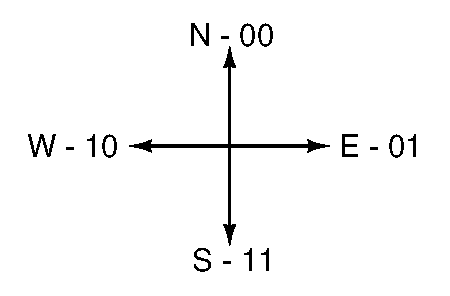
\includegraphics[scale=0.7]{numbers/gray.eps}
	\caption{This figure shows using Gray codes to represent the cardinal directions.}
	\label{fig:graydir}
\end{figure} 

Counting systems like this are called Gray code after \href{https://en.wikipedia.org/wiki/Gray_code}{Frank Gray} 
or reflected binary code. A 4-bit example is shown in Table \ref{table:graycode}.

\begin{table}[!ht]
	\centering
	\begin{tabular}{c}
		\hline
		{Gray Code}   \\ 
		\hline
		0000 \\
		0001 \\
		0011 \\
		0010 \\
		\hline
		0110 \\
		0111 \\
		0101 \\
		0100 \\
		\hline
		1100 \\
		1101 \\
		1111 \\
		1110 \\
		1010 \\
		1011 \\
		1001 \\
		1000 \\
		\hline
	\end{tabular}
	\caption{This table shows 4-bit Gray codes with horizontal lines showing the break for 2- and 3-bit Gray codes.}
	\label{table:graycode}
\end{table}

\section{Binary Background}
Originally, computers were just a bunch of switches, therefore, they only had two positions: on and off. 
This also has the benefit that there is a large amount of noise immunity. A repeater (buffer) can eliminate 
by recreating the original signal without noise. These are all great benefits of the binary system.
